% Options for packages loaded elsewhere
\PassOptionsToPackage{unicode}{hyperref}
\PassOptionsToPackage{hyphens}{url}
%
\documentclass[
]{book}
\usepackage{amsmath,amssymb}
\usepackage{iftex}
\ifPDFTeX
  \usepackage[T1]{fontenc}
  \usepackage[utf8]{inputenc}
  \usepackage{textcomp} % provide euro and other symbols
\else % if luatex or xetex
  \usepackage{unicode-math} % this also loads fontspec
  \defaultfontfeatures{Scale=MatchLowercase}
  \defaultfontfeatures[\rmfamily]{Ligatures=TeX,Scale=1}
\fi
\usepackage{lmodern}
\ifPDFTeX\else
  % xetex/luatex font selection
\fi
% Use upquote if available, for straight quotes in verbatim environments
\IfFileExists{upquote.sty}{\usepackage{upquote}}{}
\IfFileExists{microtype.sty}{% use microtype if available
  \usepackage[]{microtype}
  \UseMicrotypeSet[protrusion]{basicmath} % disable protrusion for tt fonts
}{}
\makeatletter
\@ifundefined{KOMAClassName}{% if non-KOMA class
  \IfFileExists{parskip.sty}{%
    \usepackage{parskip}
  }{% else
    \setlength{\parindent}{0pt}
    \setlength{\parskip}{6pt plus 2pt minus 1pt}}
}{% if KOMA class
  \KOMAoptions{parskip=half}}
\makeatother
\usepackage{xcolor}
\usepackage[margin=1in]{geometry}
\usepackage{color}
\usepackage{fancyvrb}
\newcommand{\VerbBar}{|}
\newcommand{\VERB}{\Verb[commandchars=\\\{\}]}
\DefineVerbatimEnvironment{Highlighting}{Verbatim}{commandchars=\\\{\}}
% Add ',fontsize=\small' for more characters per line
\newenvironment{Shaded}{}{}
\newcommand{\AlertTok}[1]{\textcolor[rgb]{1.00,0.00,0.00}{\textbf{#1}}}
\newcommand{\AnnotationTok}[1]{\textcolor[rgb]{0.38,0.63,0.69}{\textbf{\textit{#1}}}}
\newcommand{\AttributeTok}[1]{\textcolor[rgb]{0.49,0.56,0.16}{#1}}
\newcommand{\BaseNTok}[1]{\textcolor[rgb]{0.25,0.63,0.44}{#1}}
\newcommand{\BuiltInTok}[1]{\textcolor[rgb]{0.00,0.50,0.00}{#1}}
\newcommand{\CharTok}[1]{\textcolor[rgb]{0.25,0.44,0.63}{#1}}
\newcommand{\CommentTok}[1]{\textcolor[rgb]{0.38,0.63,0.69}{\textit{#1}}}
\newcommand{\CommentVarTok}[1]{\textcolor[rgb]{0.38,0.63,0.69}{\textbf{\textit{#1}}}}
\newcommand{\ConstantTok}[1]{\textcolor[rgb]{0.53,0.00,0.00}{#1}}
\newcommand{\ControlFlowTok}[1]{\textcolor[rgb]{0.00,0.44,0.13}{\textbf{#1}}}
\newcommand{\DataTypeTok}[1]{\textcolor[rgb]{0.56,0.13,0.00}{#1}}
\newcommand{\DecValTok}[1]{\textcolor[rgb]{0.25,0.63,0.44}{#1}}
\newcommand{\DocumentationTok}[1]{\textcolor[rgb]{0.73,0.13,0.13}{\textit{#1}}}
\newcommand{\ErrorTok}[1]{\textcolor[rgb]{1.00,0.00,0.00}{\textbf{#1}}}
\newcommand{\ExtensionTok}[1]{#1}
\newcommand{\FloatTok}[1]{\textcolor[rgb]{0.25,0.63,0.44}{#1}}
\newcommand{\FunctionTok}[1]{\textcolor[rgb]{0.02,0.16,0.49}{#1}}
\newcommand{\ImportTok}[1]{\textcolor[rgb]{0.00,0.50,0.00}{\textbf{#1}}}
\newcommand{\InformationTok}[1]{\textcolor[rgb]{0.38,0.63,0.69}{\textbf{\textit{#1}}}}
\newcommand{\KeywordTok}[1]{\textcolor[rgb]{0.00,0.44,0.13}{\textbf{#1}}}
\newcommand{\NormalTok}[1]{#1}
\newcommand{\OperatorTok}[1]{\textcolor[rgb]{0.40,0.40,0.40}{#1}}
\newcommand{\OtherTok}[1]{\textcolor[rgb]{0.00,0.44,0.13}{#1}}
\newcommand{\PreprocessorTok}[1]{\textcolor[rgb]{0.74,0.48,0.00}{#1}}
\newcommand{\RegionMarkerTok}[1]{#1}
\newcommand{\SpecialCharTok}[1]{\textcolor[rgb]{0.25,0.44,0.63}{#1}}
\newcommand{\SpecialStringTok}[1]{\textcolor[rgb]{0.73,0.40,0.53}{#1}}
\newcommand{\StringTok}[1]{\textcolor[rgb]{0.25,0.44,0.63}{#1}}
\newcommand{\VariableTok}[1]{\textcolor[rgb]{0.10,0.09,0.49}{#1}}
\newcommand{\VerbatimStringTok}[1]{\textcolor[rgb]{0.25,0.44,0.63}{#1}}
\newcommand{\WarningTok}[1]{\textcolor[rgb]{0.38,0.63,0.69}{\textbf{\textit{#1}}}}
\usepackage{longtable,booktabs,array}
\usepackage{calc} % for calculating minipage widths
% Correct order of tables after \paragraph or \subparagraph
\usepackage{etoolbox}
\makeatletter
\patchcmd\longtable{\par}{\if@noskipsec\mbox{}\fi\par}{}{}
\makeatother
% Allow footnotes in longtable head/foot
\IfFileExists{footnotehyper.sty}{\usepackage{footnotehyper}}{\usepackage{footnote}}
\makesavenoteenv{longtable}
\usepackage{graphicx}
\makeatletter
\def\maxwidth{\ifdim\Gin@nat@width>\linewidth\linewidth\else\Gin@nat@width\fi}
\def\maxheight{\ifdim\Gin@nat@height>\textheight\textheight\else\Gin@nat@height\fi}
\makeatother
% Scale images if necessary, so that they will not overflow the page
% margins by default, and it is still possible to overwrite the defaults
% using explicit options in \includegraphics[width, height, ...]{}
\setkeys{Gin}{width=\maxwidth,height=\maxheight,keepaspectratio}
% Set default figure placement to htbp
\makeatletter
\def\fps@figure{htbp}
\makeatother
\usepackage{soul}
\setlength{\emergencystretch}{3em} % prevent overfull lines
\providecommand{\tightlist}{%
  \setlength{\itemsep}{0pt}\setlength{\parskip}{0pt}}
\setcounter{secnumdepth}{-\maxdimen} % remove section numbering
\setkeys{Gin}{width=0.7\textwidth}
\makeatletter
\@ifpackageloaded{subfig}{}{\usepackage{subfig}}
\@ifpackageloaded{caption}{}{\usepackage{caption}}
\captionsetup[subfloat]{margin=0.5em}
\AtBeginDocument{%
\renewcommand*\figurename{Figure}
\renewcommand*\tablename{Table}
}
\AtBeginDocument{%
\renewcommand*\listfigurename{List of Figures}
\renewcommand*\listtablename{List of Tables}
}
\newcounter{pandoccrossref@subfigures@footnote@counter}
\newenvironment{pandoccrossrefsubfigures}{%
\setcounter{pandoccrossref@subfigures@footnote@counter}{0}
\begin{figure}\centering%
\gdef\global@pandoccrossref@subfigures@footnotes{}%
\DeclareRobustCommand{\footnote}[1]{\footnotemark%
\stepcounter{pandoccrossref@subfigures@footnote@counter}%
\ifx\global@pandoccrossref@subfigures@footnotes\empty%
\gdef\global@pandoccrossref@subfigures@footnotes{{##1}}%
\else%
\g@addto@macro\global@pandoccrossref@subfigures@footnotes{, {##1}}%
\fi}}%
{\end{figure}%
\addtocounter{footnote}{-\value{pandoccrossref@subfigures@footnote@counter}}
\@for\f:=\global@pandoccrossref@subfigures@footnotes\do{\stepcounter{footnote}\footnotetext{\f}}%
\gdef\global@pandoccrossref@subfigures@footnotes{}}
\@ifpackageloaded{float}{}{\usepackage{float}}
\floatstyle{ruled}
\@ifundefined{c@chapter}{\newfloat{codelisting}{h}{lop}}{\newfloat{codelisting}{h}{lop}[chapter]}
\floatname{codelisting}{Listing}
\newcommand*\listoflistings{\listof{codelisting}{List of Listings}}
\makeatother
\ifLuaTeX
  \usepackage{selnolig}  % disable illegal ligatures
\fi
\IfFileExists{bookmark.sty}{\usepackage{bookmark}}{\usepackage{hyperref}}
\IfFileExists{xurl.sty}{\usepackage{xurl}}{} % add URL line breaks if available
\urlstyle{same}
\hypersetup{
  pdftitle={Artificial Intelligence Techniques - Lecture Notes},
  pdfauthor={Zohar Cochavi},
  hidelinks,
  pdfcreator={LaTeX via pandoc}}

\title{Artificial Intelligence Techniques - Lecture Notes}
\usepackage{etoolbox}
\makeatletter
\providecommand{\subtitle}[1]{% add subtitle to \maketitle
  \apptocmd{\@title}{\par {\large #1 \par}}{}{}
}
\makeatother
\subtitle{Notes to aid, not to replace. I'm simply a human, thus the
risk you embrace.}
\author{Zohar Cochavi}
\date{}

\begin{document}
\frontmatter
\maketitle

\mainmatter
\hypertarget{introduction}{%
\chapter{Introduction}\label{introduction}}

Not much needs to be said regarding the introduction of probabilistic
machine learning. However, one rule deserves special attention and a
quick reminder is therefore in place.

\hypertarget{bayes-rule}{%
\section{Bayes' Rule}\label{bayes-rule}}

In short, Bayes' rule allows us to `update' our current belief, i.e.~the
probability of a state, \(S\) given some possible actions,
\(a_0, \ldots, a_i\), \(P(S | a_0, \ldots, a_i)\), using observations.
That is, by `flipping' the dependence, actions given the next state
instead of the next state given actions, we can relate actions and
states.

Let me clarify by first providing Bayes' rule:

\begin{equation}\protect\hypertarget{eq:bayes-rule}{}{
P(S|a) = \frac{P(a|S)P(S)}{P(a)}
}\label{eq:bayes-rule}\end{equation}

Instead of using \(a\) for action, we can also use \(o\) for
observation. When considering a classification example, this makes more
sense. In that case, we would like to `learn' how certain attributes
relate to classes (the states in the previous example). This is done by
making `observations' in the form of features and, since we already have
the label, this results in \emph{an observation given some label}. Using
Bayes' theorem (see eq.~\ref{eq:bayes-rule}), we can thus determine the
\emph{label given some features}.

The example of actions and states applies when considering an
\textbf{agent} acting in an unfamiliar environment. Here, we consider
\(P(S)\) our \textbf{prior} belief, or the belief before (prior to) the
observation, and `update' the belief by considering our belief given
some observations, \(P(S|o)\).

This implies somehow that \(P(o|S)\) is easier to determine than its
inverse. {[}\ldots{]}

\hypertarget{imitation-learning---inverse-reinforcement-learning}{%
\chapter{Imitation Learning - Inverse Reinforcement
Learning}\label{imitation-learning---inverse-reinforcement-learning}}

\begin{itemize}
\tightlist
\item
  Instead of learning everything ourselves, we want to use some expert
  examples and improve from there. This is called \textbf{imitation
  learning} or \textbf{behavioral cloning}.
\item
  One technique for applying such learning is \textbf{inverse
  reinforcement learning} in which the model attempts to find the
  rewards associated with certain actions.
\end{itemize}

\begin{longtable}[]{@{}
  >{\raggedright\arraybackslash}p{(\columnwidth - 14\tabcolsep) * \real{0.1250}}
  >{\raggedright\arraybackslash}p{(\columnwidth - 14\tabcolsep) * \real{0.1250}}
  >{\raggedright\arraybackslash}p{(\columnwidth - 14\tabcolsep) * \real{0.1250}}
  >{\raggedright\arraybackslash}p{(\columnwidth - 14\tabcolsep) * \real{0.1250}}
  >{\raggedright\arraybackslash}p{(\columnwidth - 14\tabcolsep) * \real{0.1250}}
  >{\raggedright\arraybackslash}p{(\columnwidth - 14\tabcolsep) * \real{0.1250}}
  >{\raggedright\arraybackslash}p{(\columnwidth - 14\tabcolsep) * \real{0.1250}}
  >{\raggedright\arraybackslash}p{(\columnwidth - 14\tabcolsep) * \real{0.1250}}@{}}
\caption{Various methods for imitation learning and their different
attributes\{\#tbl:imitation\_learning\}}\tabularnewline
\toprule\noalign{}
\begin{minipage}[b]{\linewidth}\raggedright
\end{minipage} & \begin{minipage}[b]{\linewidth}\raggedright
Direct Policy Learning
\end{minipage} & \begin{minipage}[b]{\linewidth}\raggedright
Reward Learning
\end{minipage} & \begin{minipage}[b]{\linewidth}\raggedright
Access to Environment
\end{minipage} & \begin{minipage}[b]{\linewidth}\raggedright
Interactive Demonstrator
\end{minipage} & \begin{minipage}[b]{\linewidth}\raggedright
Pre-collected demonstrations
\end{minipage} & \begin{minipage}[b]{\linewidth}\raggedright
\end{minipage} & \begin{minipage}[b]{\linewidth}\raggedright
\end{minipage} \\
\midrule\noalign{}
\endfirsthead
\toprule\noalign{}
\begin{minipage}[b]{\linewidth}\raggedright
\end{minipage} & \begin{minipage}[b]{\linewidth}\raggedright
Direct Policy Learning
\end{minipage} & \begin{minipage}[b]{\linewidth}\raggedright
Reward Learning
\end{minipage} & \begin{minipage}[b]{\linewidth}\raggedright
Access to Environment
\end{minipage} & \begin{minipage}[b]{\linewidth}\raggedright
Interactive Demonstrator
\end{minipage} & \begin{minipage}[b]{\linewidth}\raggedright
Pre-collected demonstrations
\end{minipage} & \begin{minipage}[b]{\linewidth}\raggedright
\end{minipage} & \begin{minipage}[b]{\linewidth}\raggedright
\end{minipage} \\
\midrule\noalign{}
\endhead
\bottomrule\noalign{}
\endlastfoot
Behavioral cloning (BC) & Yes & No & No & No & Yes & & \\
Direct policy learning (interactive IL) & Yes & No & Yes & Yes &
Optional & & \\
Inverse Reinforcement Learning (IRL) & No & Yes & Yes & No & Yes & & \\
Preference-based RL & No & Yes & Yes & Yes & No & & \\
\end{longtable}

\begin{itemize}
\item
  The formal goal is as follows: find a reward function \(R\) for which
  the expert-provided policy is optimal.
\item
  This, however, is a rather `vague' solution for which some heuristics
  will make developing a general solution a little easier:

  \begin{enumerate}
  \def\labelenumi{\arabic{enumi}.}
  \tightlist
  \item
    We prefer solutions where the distance (the difference in value is
    maximal) to other policies: \(\max_{R}(\pi^*_R - \pi_R)\)
  \item
    We prefer smaller rewards: \(\min(R)\) or \(\max(-R)\).
  \end{enumerate}
\end{itemize}

\hypertarget{bayesian-networks-and-inference}{%
\chapter{Bayesian Networks and
Inference}\label{bayesian-networks-and-inference}}

Core to the idea of an intelligent agent is that the agent somehow
manages to solve a task for which the solution is not explicitly
embedded into the agent. If we told the agent explicitly what to do, it
would simply be a front for some deterministic algorithm. The lack of
determinism therefore implies the need for the agent to handle
uncertainty. Therefore, we need to be able to formally represent
uncertainty.

More formally, an issue arises when an agent attempts to determine
whether it will be able to complete a task. It might guarantee a certain
outcome, \emph{given} that a whole host of events do, or do not, take
place. This just kicks the can down the road, as we then have to
guarantee whether the dependencies for the result are also satisfied.
This leads to something called the \textbf{qualification problem}.

Combining some fundamental intuition about probability and the issue of
the qualification problem, we can look at events as a chain of
probabilistic dependencies. One way of structuring such dependencies is
in something called a \textbf{Bayesian Network}.

\hypertarget{representing-knowledge-in-an-uncertain-domain}{%
\section{Representing Knowledge in an Uncertain
Domain}\label{representing-knowledge-in-an-uncertain-domain}}

A Bayesian Network is a data structure that encapsulates the full joint
probability distribution in a concise manner. Meaning it is nothing more
than a representation of a (possibly very complex) function. Let's take
the example of a patient having a cavity in their tooth, \(P(Cavity)\)
which might induce a toothache and can be observed with a `catch' (see
fig.~\ref{fig:cavity-graph}).

\hypertarget{fig:cavity-graph}{%
\label{fig:cavity-graph}}%
\begin{Shaded}
\begin{Highlighting}[]
\NormalTok{graph TD;}
\NormalTok{    Cavity{-}{-}\textgreater{}Toothache;}
\NormalTok{    Cavity{-}{-}\textgreater{}Catch;}
\NormalTok{    Weather;}
\end{Highlighting}
\end{Shaded}

There, we see how one random variable might influence two other random
variables. Furthermore, there is no need for all the nodes to be
connected, a forest is a valid instance of a Bayesian network (the
weather is independent of the cavity).

There is another assumption hidden in this graph, namely that
\(Toothache\) and \(Catch\) are \textbf{conditionally independent} given
\(Cavity\). Conditional independence is formalized by the following
relation.

\[
P(Catch \land Toothache | Cavity) = P(Catch | Cavity) \land P(Toothache |
Cavity)
\]

A formal specification of a Bayesian Network (BN) can be characterized
as follows:

\begin{enumerate}
\def\labelenumi{\arabic{enumi}.}
\tightlist
\item
  Each node corresponds to a random variable, which may be discrete or
  continuous.
\item
  A set of directed links or arrows connects pairs of nodes. If there is
  an arrow from node \(X\) to node \(Y\), \(X\) is said to be a parent
  of \(Y\). The graph has no directed cycles (and hence is a directed
  acyclic graph, or DAG).
\item
  Each node \(X_i\) has a conditional probability distribution
  \(P(X_i | Parents(X_i))\) that quantifies the effect of the parents on
  the node.
\end{enumerate}

A more involved example would be the following, where an \(Alarm\) might
be triggered by \(Burglary\) or an \(Earthquake\) which then proceeds to
call John, \(JohnCalls\), or Mary, \(MaryCalls\).

\hypertarget{fig:alarm}{%
\label{fig:alarm}}%
\begin{Shaded}
\begin{Highlighting}[]
\NormalTok{graph TD;}
\NormalTok{    Burglary {-}{-}{-}\textgreater{} Alarm;}
\NormalTok{    Earthquake {-}{-}{-}\textgreater{} Alarm;}
\NormalTok{    Alarm {-}{-}{-}\textgreater{} JohnCalls;}
\NormalTok{    Alarm {-}{-}{-}\textgreater{} MaryCalls;}
\end{Highlighting}
\end{Shaded}

The \textbf{conditional probability table} (CPT) of \(Alarm\) can be
found in tbl.~\ref{tbl:cpt}. Since we are dealing with binary conditions
(either \(A\) happens or it doesn't), \(P(\not A)\) is implicit. In
other cases, the sum of the probabilities in one row should equal \(1\)
to be considered valid probabilities.

\hypertarget{tbl:cpt}{}
\begin{longtable}[]{@{}ccl@{}}
\caption{\label{tbl:cpt}Conditional probability table (CPT) of the
\(Alarm\) event. Notice how dependence increases the size of the table
according to \(2^n\), where \(n\) is the number of dependent variables.
This is because we are dealing with Boolean conditions.}\tabularnewline
\toprule\noalign{}
B & E & P(A) \\
\midrule\noalign{}
\endfirsthead
\toprule\noalign{}
B & E & P(A) \\
\midrule\noalign{}
\endhead
\bottomrule\noalign{}
\endlastfoot
t & t & .95 \\
t & f & .94 \\
f & t & .29 \\
f & f & .001 \\
\end{longtable}

\hypertarget{the-semantics-of-bayesian-networks}{%
\section{The Semantics of Bayesian
Networks}\label{the-semantics-of-bayesian-networks}}

As mentioned before, a BN is a representation of a joint distribution
function. Another way to interpret it, however, is to view it as an
encoding of a collection of conditional independence statements. Instead
of focusing on how one is dependent on another, we think about which
events are \emph{not} dependent on another.

A BN can be described and used according to the following relation,
which stems from the \textbf{chain rule}.

\[
P(x_1, \ldots, x_n) = \prod^n_{i=1} P(x_i|parents(X_i))
\]

That is, the probability of a certain set of outcomes for the events
described by the BN (i.e.~the values of it's nodes) can be calculated by
taking the product of the probabilities of all these events given their
respective parent(s). The conditional probability used in the product
series can then be described by the aforementioned CPT.

This means that, even though the BN is technically equivalent to the
joint probability distribution, assuming the network is sparse (i.e.~not
all nodes are connected to all other nodes) it is more efficient in
terms of computation. Consider the following: if a joint probability
distribution of Boolean random variables scales according to \(2^n\)
where \(n\) is the number of random variables, a BN scales according to
\(n2^k\) where \(k\) is the average number of parents.

Formally, we can say that a node is conditionally independent of its
\textbf{non-descendents} given its parents. Furthermore, we can say that
a node is conditionally independent of the whole network given its
parents, children, and children's parents, also called its
\textbf{Markov Blanket}. The more connected a BN is, the bigger the
average Markov Blanket of its nodes.

Instead of considering all combinations of events, we assume that some
events do not influence one another. At the core of the BN lies this
assumption, and one should therefore consider the balance between
accuracy and computational complexity.

\hypertarget{efficient-representation-of-conditional-distributions}{%
\section{Efficient Representation of Conditional
Distributions}\label{efficient-representation-of-conditional-distributions}}

Assumptions can be made about the interaction of parents and how they
relate to their children. We can assume logical or min/max statements,
and from there construct the complete CPT. An example would be a
\(Fever\) which could be caused by the \(Flu\), a \(Cold\), or
\(Malaria\). We then assume that these relate to each other in something
called a \textbf{fuzzy OR} scenario, i.e.~the relation tends to that of
a logical OR. This means that we would only need, for example, the
probability of someone to get a \(Fever\) from the \(Cold\) and the
probability to get a \(Fever\) from the \(Flu\) to determine what the
combined probability (see eq.~\ref{eq:fever})

\begin{equation}\protect\hypertarget{eq:fever}{}{
\begin{gathered}
P(Fever | Cold, Flu, \neg Malaria) = \\
(1 - P(\neg Fever | Cold, \neg Flu, \neg Malaria) \cdot P(\neg Fever | \neg Cold, Flu, \neg Malaria))
\end{gathered}
}\label{eq:fever}\end{equation}

Instead of using a CPT, we can also employ `normal' probability density
functions (PDFs) to describe the probabilistic characteristics of a
random variable. While we could use discretization to work with
continious random variables, this often comes at a loss of accuracy and
potentially unwieldy CPTs. There are some considerations to make with
regard to \textbf{hybrid networks} where we find both discrete and
continuous random variables. Most notably, when a continuous parent has
a discrete child, we have to create some threshold function. The most
interesting here is the so-called \textbf{logistic function} which is
often used in neural networks for the same purpose.

\hypertarget{bowtie-exact-inference}{%
\section{\texorpdfstring{\(\bowtie\) Exact
Inference}{\textbackslash bowtie Exact Inference}}\label{bowtie-exact-inference}}

Now my friends, the time has come, to collect info and probably infer
some. We know how BNs work and how to construct them. Now, we would like
to use our model to infer information given some state, i.e.~perform a
query.

In this section, we will only discuss \emph{exact} inference. First, we
discuss the `easy' way, and then apply some optimization on top of that
in the form of memoization.

\hypertarget{inference-by-enumeration}{%
\subsection{Inference by Enumeration}\label{inference-by-enumeration}}

Let's take the BN presented in fig.~\ref{fig:alarm}, and use the
following query: \(P(Burglary\ |\ JohnCalls = true, MaryCalls = true)\).
Inference by enumeration simply takes all the possible contexts in which
John might call, and where Mary might call and considers where this
would have been caused by a burglary.

We can start solving our query using the following relation,

\[
P(X\ |\ e) = \alpha P(X, e) = \alpha \sum_y P(X, e, y)
\]

where \(\alpha=\frac{1}{e}\).

Applying our query to the equation then gives,

\[
P(B\ |\ j, m) = \alpha P(B, j, m) = \alpha \sum_e \sum_a P(B, j, m, e, a)
\]

For the sake of simplicity, we only consider \(B=true\), which can be
rewritten to the following when taking our BN as the joint function
(i.e.~substitute \(P(B, j, m, e, a\) with the characteristic of the BN).

\[
P(b\ |\ j, m) = \alpha \sum_e \sum_a P(b)P(e)P(a\ |\ b,e)P(j\ |\ a)P(m\ |\ a)
\]

Which can then be simplified as follows,

\begin{equation}\protect\hypertarget{eq:enumeration}{}{
P(b\ |\ j, m) = \alpha P(b) \sum_e P(e) \sum_a P(a\ |\ b,e)P(j\ |\ a)P(m\ |\ a)
}\label{eq:enumeration}\end{equation}

and then be solved by looking up the respective values in the CPTs.

\hypertarget{variable-elimination}{%
\subsection{Variable Elimination}\label{variable-elimination}}

One can imagine the previous algorithm to be suboptimal. Considering the
time complexity, we come to the conclusion that it runs in
\(\mathcal{O}(2^n)\). Realizing your algorithm runs in exponential time
is never a nice experience.. But, it's a great improvement considering
calculating the straight joint probability runs in
\(\mathcal{O}(n2^n)\).

One way in which we can improve the performance of the model, is by
reusing past calculations (memoization, if you know, you know). This
dynamic programming technique is called \textbf{variable elimination}.
The idea is to solve the equation from the bottom up (that is, when
viewed as a syntax tree, we start at the leaves and move up) so that we
can re-use calculations we've made before.

{[}\ldots{]}

\hypertarget{maintaining-a-belief-over-time}{%
\chapter{Maintaining a Belief over
Time}\label{maintaining-a-belief-over-time}}

\hypertarget{introduction-1}{%
\section{Introduction}\label{introduction-1}}

\begin{itemize}
\tightlist
\item
  Changing the simple \textbf{sensor model} to a \textbf{transition
  model} by incorporating time steps, but no ability to which next state
  is the most likely (why? most probable is not most likely?).
\item
  Different Types of models:

  \begin{itemize}
  \tightlist
  \item
    Hidden Markov Models
  \item
    Kalman Filters
  \item
    Dynamic Bayesian Networks
  \end{itemize}
\item
  Incorporating time can be important to, for example, take into account
  the rate of change (first derivative) when making decisions.
\end{itemize}

\hypertarget{transition-and-sensor-models}{%
\section{Transition and Sensor
Models}\label{transition-and-sensor-models}}

\begin{itemize}
\tightlist
\item
  \textbf{Markov assumption}: \emph{``The current state depends on only
  a finite fixed number of previous states.''} Any system or process
  that satisfies this assumption is called a \textbf{Markov Process} or
  \textbf{Markov Chain}.
\item
  The number of dependent prior states, \(n\), is integrated into the
  so-called order, a so-called \textbf{\(n\)th-order Markdown Process}.
\item
  Formally, a first-order Markov process is denoted as:
\end{itemize}

\[
P(X_t|X_{0:t-1}) = P(X_t|X_{t-1})
\]

\begin{itemize}
\tightlist
\item
  Important is that the underlying laws of the system do not change,
  therefore, the distributions are stationary over \(t\).
\item
  Another important assumption is that of the \textbf{sensor Markov
  assumption} (see eq.~\ref{eq:sensor_markov_assumption}). That is, the
  observable variable is only dependent on the hidden variable in the
  current time-step. Also called the observation model.
\end{itemize}

\begin{equation}\protect\hypertarget{eq:sensor_markov_assumption}{}{
P(E_t|X_{0:t}, E_{0:t-1}) = P(E_t|X_t)
}\label{eq:sensor_markov_assumption}\end{equation}

\begin{itemize}
\tightlist
\item
  The process has to initialize with a prior probability at \(t=0\),
  \(P(X_0)\).
\item
  Thus, we can denote the complete joint probability distribution for a
  \textbf{first-order Markov Process} (see
  eq.~\ref{eq:first_order_markov}).
\end{itemize}

\begin{equation}\protect\hypertarget{eq:first_order_markov}{}{
P(X_{0:t}, E_{1:t}) = P(X_0) \prod^t_{i=1} P(X_i|X_{i-1})P(E_i|X_i)
}\label{eq:first_order_markov}\end{equation}

\begin{itemize}
\tightlist
\item
  The accuracy of such a model depends on how `reasonable' the Markov
  assumption is, and how closely the chain of causality resembles the
  real world (the probability that someone brings an umbrella might also
  be dependent on the amount of sun, instead of only whether it's
  raining.).
\item
  There are two ways to improve the accuracy of a model (which are
  re-formulations of one-another):

  \begin{enumerate}
  \def\labelenumi{\arabic{enumi}.}
  \tightlist
  \item
    Increase the order of the Markov process model.
  \item
    Increase the set of state variables.
  \end{enumerate}
\end{itemize}

\hypertarget{inference-in-temporal-models}{%
\section{Inference in Temporal
Models}\label{inference-in-temporal-models}}

\begin{itemize}
\tightlist
\item
  Various methods for inference exist which can complement each other to
  improve accuracy of the model besides just answering queries.

  \begin{enumerate}
  \def\labelenumi{\arabic{enumi}.}
  \tightlist
  \item
    \textbf{Filtering}: Informs our agent about the distribution of the
    current hidden state based on the observations made until now,
    \(P(X_t|e_{1:t})\).
  \item
    \textbf{Prediction}: Determine the distribution of the next hidden
    state based on the observations made until now,
    \(P(X_{t+1}|e_{1:t})\).
  \item
    \textbf{Smoothing}: Determine the distribution of a past hidden
    state, \(0 \ge k \lt t\), based on the observations made until now,
    \(P(X_k|e_{1:t})\).
  \item
    \textbf{Most likely explanation}: Determine the most likely sequence
    of events based on the observations made until now,
    \(P(x_{1:t}|e_{1:t})\).
  \end{enumerate}
\item
  Another technique called \textbf{Learning}, is based on
  \textbf{smoothing} combined with the \textbf{EM} algorithm.
\end{itemize}

\hypertarget{filtering-and-prediction}{%
\subsection{Filtering And Prediction}\label{filtering-and-prediction}}

\begin{itemize}
\tightlist
\item
  The process of filtering (see eq.~\ref{eq:filtering_markov}) depends
  on prediction, (at least, based on the formulations mentioned above).
  (\(\alpha\) is always a normalization constant).
\end{itemize}

\begin{equation}\protect\hypertarget{eq:filtering_markov}{}{
P(X_{t+1}|e_{1:t+1}) = \alpha P(e_{t+1}|X_{t+1}) \sum_{x_t} P(X_{t+1}|x_t) P(x_t|e_{1:t})
}\label{eq:filtering_markov}\end{equation}

\begin{itemize}
\item
  They are two steps that are necessary for one another. Therefore,
  while they are separate queries, they could be considered two steps in
  the same process. To get \(P(X_{t+1}|e_{1:t+1})\),

  \begin{enumerate}
  \def\labelenumi{\arabic{enumi}.}
  \tightlist
  \item
    Predict: \[
      P(X_{t+1}|e_{1:t}) = \sum_{x_{t-1}} P(X_t|x_{t-1}) P(x_{t-1})
      \]
  \item
    Filter: \[
      P(X_{t+1}|e_{1:t+1}) = \alpha P(e_{t+1}|X_{t+1}) P(X_{t+1}|e_{1:t})
      \]
  \end{enumerate}
\item
  The initialization predict step could be considered as prediction with
  empty evidence (i.e.~without evidence), \(e_0\). In which case it
  reduces to the prior, \(P(x_0|e_0) = P(x_0)\). \[
  \begin{split}
  P(X_1|e_0) &= \sum_{x_0}P(X_1|x_0)P(x_0|e_0) \\
             &= \sum_{x_0}P(X_1|x_0)P(x_0) \\
  \end{split}
  \]
\end{itemize}

\hypertarget{smoothing}{%
\subsection{Smoothing}\label{smoothing}}

\begin{itemize}
\tightlist
\item
  With smoothing, we can essentially improve the model to take into
  account new observations, and can be described by
  eq.~\ref{eq:smoothing_markov}.
\end{itemize}

\begin{equation}\protect\hypertarget{eq:smoothing_markov}{}{
\begin{split}
P(X_k|e_{1:t}) &= \alpha P(X_k|e_{1:k}) P(e_{k+1:t}|X_k) \\
               &= \alpha f_{1:k} \times b_{k+1:t}
\end{split}
}\label{eq:smoothing_markov}\end{equation}

\begin{itemize}
\tightlist
\item
  The factors \(f\) and \(b\), implying forward and backward
  respectively, can then be described by eq.~\ref{eq:filtering_markov}
  and eq.~\ref{eq:smoothing_backward} respectively.
\end{itemize}

\begin{equation}\protect\hypertarget{eq:smoothing_backward}{}{
\begin{gathered}
  P(e_{k+1:t}|X_k) = \sum_{x_{k+1}} P(e_{k+1}|x_{k+1}) P(e_{k+2:t}|x_{k+1}) P(x_{k_1}|X_k) \\
  \implies b_{k+1:t} = Backward(b_{k+2:t}, e_{k+1})
\end{gathered}
}\label{eq:smoothing_backward}\end{equation}

\begin{itemize}
\tightlist
\item
  While smoothing would take \(O(t)\) for a single time-step, and thus
  \(O(t^2)\) for all timesteps, by saving the intermediate results, we
  can smooth the whole sequence in \(O(t)\) by applying the
  \textbf{forward-backward algorithm}.
\end{itemize}

\hypertarget{most-likely-sequence}{%
\subsection{Most-likely Sequence}\label{most-likely-sequence}}

\begin{itemize}
\tightlist
\item
  Since the most-likely sequence is formed by the joint probability of
  all the hidden states, we cannot just apply smoothing and calculate
  the most likely hidden state based on that states' prior. \hl{I sort
  of get the idea why you can't just keep `smoothing' over and over
  again and then use those states, but I can't quite put my finger on
  it.}
\end{itemize}

\begin{equation}\protect\hypertarget{eq:most_likely_markov}{}{
\begin{gathered}
\max_{x_1 \ldots x_t} P(x_1, \ldots, x_t, X_{t+1} | e_{1:t+1}) \\
= \alpha P(e_{t+1}|X_{t+1}) \max_{x_t}
 \left( P(X_{t+1}|x_t) \max_{x_1 \ldots
x_{t-1}} P(x_1, \ldots, x_{t-1}, x_t | e_{1:t}) \right)
\end{gathered}
}\label{eq:most_likely_markov}\end{equation}

\begin{itemize}
\tightlist
\item
  The algorithm to compute the most likely sequence is also called the
  \textbf{Viterbi algorithm} (see eq.~\ref{eq:most_likely_markov}).
\end{itemize}

\hypertarget{dynamic-bayesian-networks}{%
\section{Dynamic Bayesian Networks}\label{dynamic-bayesian-networks}}

\begin{itemize}
\tightlist
\item
  Dynamic Bayesian Networks (DBNs) are a generalization of the HMMs.
  Every HMM is a single-variable DBN; every discrete DBN is an HMM.
  \textbf{A DBN can have multiple `sensors', while a HMM can have only
  one} (that is one observable).
\item
  Exact inference in DBNs becomes intractable as their size grows. Thus,
  we use approximate inference. Specifically, \textbf{particle
  filtering}:
\end{itemize}

\begin{quote}
First, a population of \(N\) initial-state samples is created by
sampling from the prior distribution \(P(X_0)\). Then, the update cycle
is repeated for each time step:

\begin{enumerate}
\def\labelenumi{\arabic{enumi}.}
\tightlist
\item
  Each sample is propagated forward by sampling the next state value
  \(x_{t+1}\) given the current value \(x_t\) for the sample, based on
  the transition model \(P(X_{t+1}|x_t)\).
\item
  Each sample is weighted by the likelihood it assigns to the new
  evidence, \(P(e_{t+1}| x_{t+1})\)
\item
  The population is resampled to generate a new population of \(N\)
  sample. Each new sample is selected from the current population; the
  probability that a particular sample is selected is proportional to
  its weight. The new samples are unweighted.
\end{enumerate}
\end{quote}

\hypertarget{learning}{%
\chapter{Learning}\label{learning}}

\hypertarget{why-learning}{%
\section{Why Learning}\label{why-learning}}

\begin{enumerate}
\def\labelenumi{\arabic{enumi}.}
\item
  Some model might not be available. In this case, it can be built up
  over time by some other algorithm. An example would be to train a deep
  learning model; there is no \emph{specific} version of the model
  available to the programmers, but we can adapt a general model to our
  specific purposes.
\item
  \ldots{}
\item
  Not understanding the problem.
\end{enumerate}

\hypertarget{what-is-learning}{%
\section{What is learning}\label{what-is-learning}}

While there are many approaches to learning, some of which might be more
useful/correct in certain contexts than others. Here, we focus on
\textbf{learning as induction}. How to use induction to learn is then
dependent on the technique that is used to implement some agent.

Thus, while were are not explicitly building a model, we provide
information to some statistical model to then make decisions. It is
therefore important to decided what kind of information we should
provide the model for it to make the right decision. Not only that, we
also have to quantify what is the right decision.

We can split the space of what is the `right' decision into two
philosophies, the \textbf{Idealistic} and \textbf{Pragmatic} approach.
The idealistic attempts to stay true to the way the world works, making
observations and then using statistical models to learn. The pragmatic
approach, however, simply considers ``whatever improves the
performance''.

While the idealistic perspective would have great accuracy, the
tractability, however, is at odds. As the world is incredibly complex,
the search space for hypothesis (often denoted as \(H\)) is also
\emph{huge}. Therefore, assumptions often need to be made, which brings
most, if not any, model somewhere in between the two extremes.

\hypertarget{formalizing-learning}{%
\section{Formalizing Learning}\label{formalizing-learning}}

\begin{itemize}
\item
  Learning in Bayesian Networks can take a couple of forms:

  \begin{enumerate}
  \def\labelenumi{\arabic{enumi}.}
  \item
    \textbf{Bayesian Learning}: Is done by computing the posterior
    \(P(H|o)\) which uses the prior \(P(h)\) and can be used in a
    weighted variant (utility) to determine the best `action',
    \(V(a) = \sum_h P(H|d)u(a, h)\)

    \begin{itemize}
    \tightlist
    \item
      Bayesian learning is optimal, but untractable with realistic
      scenarios as the hypothesis space is often incredibly large.
    \end{itemize}
  \item
    \textbf{Maximum Likelihood}: The most likely hypothesis, \(h_{ML}\)
    will be \(h_{ML} = \max_h P(d|h)\). Then we can select and action
    according to \(V(a) = u(a, h_{ML})\). It is, however, prone to
    overfitting.

    \begin{itemize}
    \item
      Instead of computing the default maximum likelihood, we often
      compute the maximum \textbf{log likelihood}. As the logarithm is a
      monotonically increasing function, it should preserve the maxima
      we are looking for.
    \item
      For example, the equation
      \(P(d|h_\theta) = \theta^c \cdot (1 - \theta)^l\), where \(c\) is
      the number of cherry candies, \(l\) the number of lime candies and
      \(\theta\) the probability of encountering the former, can be
      solved in a more `computationally friendly' manner by taking the
      log, \(L(d|h_\theta) = c \log \theta + l \log (1-\theta)\). We can
      then find the maximum by taking the derivative and finding \(0\),
      \(\frac{d L(d|h_\theta)}{d\theta}=0\). This will result in
      \(\theta = \frac{c}{c + l}\), not very surprising.
    \end{itemize}
  \item
    \textbf{Maximum A Posteriori (MAP)}: Which is just the \textbf{ML},
    but also taking into consideration the prior of the hypothesis:
    \(h_{MAP} = \max_h P(d|h)P(h)\).

    \begin{itemize}
    \tightlist
    \item
      Here, the prior (just like in Bayesian Learning) penalizes the
      hypothesis being too complex. We regard more complex hypotheses
      being less likely.
    \end{itemize}
  \end{enumerate}
\item
  To be clear, this is distinct from \textbf{Most Likely Sequence
  Estimation} because there, we attempt to determine what happened, but
  the model itself doesn't necessarily improve. We learn about hidden
  states, but nothing about the model. \hl{This is my current hypothesis
  as of lecture 5}
\end{itemize}

\hypertarget{the-em-algorithm}{%
\subsection{The EM Algorithm}\label{the-em-algorithm}}

\begin{itemize}
\item
  Before, we only considered learning when we had access to data about
  \emph{all} the relevant variables. Now, we consider learning not only
  the observable data, but also hidden or \textbf{latent variables}.
\item
  To solve such learning problems, one can use the \textbf{Expectation
  Maximization} algorithm, or, \textbf{EM Algorithm}.
\item
  Take the problem of learning \textbf{mixture of Gaussians} (we will
  later see how this is relevant to latent variables). That is, we have
  a \textbf{mixture distrbution}, \(P\), with \(k\) \textbf{components}:
\end{itemize}

\[
P(x) = \sum_k P(C=i)P(x|C=i)
\]

\begin{itemize}
\item
  The problem then is, \emph{determine the center, \(\mu_i\), of each
  Gaussian and the covariance, \(\Sigma_i\), of each component, \(i\)}.
\item
  The EM algorithm will provide exactly this and works according to a
  two-step process.

  \begin{enumerate}
  \def\labelenumi{\arabic{enumi}.}
  \tightlist
  \item
    \textbf{E-step}: Compute probabilities \(p_{ij} = P(C=i|x_j)\), the
    probability that datum \(x_j\) was generated by component \(i\). By
    Bayes' rule, we have \(p_{ij}=\alpha P(x_j|C=i)P(C=i)\). The term
    \(P(x_j|C=i)\) is just the probabiltiy at \(x_j\) for the \(i\)th
    Gaussian. Define \(n_i=\sum_j p_{ij}\), the effective number of data
    points currently assigned to component \(i\).
  \item
    \textbf{M-step}: Compute the new mean, covariance, and component
    weights using the following steps in sequence:
  \end{enumerate}
\end{itemize}

\[
\begin{split}
   \mu_i &\leftarrow \sum_j p_ij x_j / n_i \\
   \Sigma_i &\leftarrow \sum_j p_ij (x_j - \mu_i)(x_j - \mu_i)^T / n_i \\
   w_i &\leftarrow n_i / N
\end{split}
\]

\hypertarget{quantification-of-objectives-and-reward-hacking}{%
\chapter{Quantification of Objectives and Reward
Hacking}\label{quantification-of-objectives-and-reward-hacking}}

\begin{itemize}
\tightlist
\item
  AI can be viewed as a model that is optimized according to a function
  that reflects 'intelligent behavior. (Backpropagation, Reinforcement
  Learning, Genetic Algorithms, etc.)
\end{itemize}

\hypertarget{fitness-and-quantification}{%
\section{Fitness and Quantification}\label{fitness-and-quantification}}

\begin{itemize}
\item
  This `fitness' has to be adjusted based on the problem at hand. For
  example,

  \begin{itemize}
  \tightlist
  \item
    Sum of squared errors for regression.
  \item
    \emph{Cross-entropy} for classification (i.e.~difference between two
    probability distributions).
  \end{itemize}
\item
  Because we want to compute how our `current' model compares to
  previous ones, we want the function to be quantifiable. That is,
  quantifiable in both input and output. \hl{(not quite the right use of
  quantifiable)}
\item
  Quantifying is hard because you embed assumptions about the problem
  you are trying to solve in the data you supply to the algorithm, and
  \emph{the algorithm is only as good as the data you supply it with}.
\end{itemize}

\hypertarget{reward-hacking}{%
\section{Reward Hacking}\label{reward-hacking}}

\begin{itemize}
\tightlist
\item
  \textbf{Reward Hacking}, or the \textbf{Inner Alignment} problem:
\end{itemize}

\begin{quote}
The objective function admits some clever ``easy'' solution that
formally maximizes it but perverts the spirit of the designer's intent
(i.e.~the objective function can be ``gamed'')
\end{quote}

\begin{itemize}
\tightlist
\item
  \textbf{Goodhart's law} puts this behavior into perspective and
  reminds us that this is similar to human behavior:
\end{itemize}

\begin{quote}
Any observed statistical regularity will tend to collapse once pressure
is placed upon it for control purposes.

When a measure becomes a target, is ceases to be a good measure.
\end{quote}

\begin{itemize}
\item
  Several reasons could exist for an agent not displaying the
  expected/desired behavior that are associated with reward hacking:

  \begin{enumerate}
  \def\labelenumi{\arabic{enumi}.}
  \tightlist
  \item
    The objective function is wrong.
  \item
    The objective function is not properly evaluated (implementation or
    other practical issue besides the mathematical basis).
  \item
    The objective is `correct', but the agent could not learn the
    `correct behavior'.
  \end{enumerate}
\item
  All these concepts might be responsible for agents acting out. It's
  important to consider that \emph{someone} has to then take
  responsibility for these problems.
\end{itemize}

\hypertarget{meaningful-human-control-over-ai}{%
\section{Meaningful Human Control over
AI}\label{meaningful-human-control-over-ai}}

\begin{quote}
\emph{Humans} not computers and their algorithms should ultimately
remain in control of, and thus be \emph{morally responsible} for
relevant decisions.
\end{quote}

\begin{itemize}
\tightlist
\item
  One approach to ensure humans can still bear responsibility to these
  systems, is to consider the \textbf{tracking} and \textbf{tracing}
  conditions:
\end{itemize}

\begin{quote}
\textbf{Tracking}: The human-AI system (consisting of human agents, AI
agents, infrastructures, etc.) should be able to track the relevant
moral reasons of the relevant human agent(s) and be responsive to these
reasons.

\textbf{Tracing}: The system's behavior should be traceable to at least
one human in the system design history or use context who can appreciate
the capabilities of the system and their own role as morally
responsible.
\end{quote}

\begin{itemize}
\tightlist
\item
  Tracking and tracing can be further quantified into the following
  properties:

  \begin{enumerate}
  \def\labelenumi{\arabic{enumi}.}
  \tightlist
  \item
    The system has an explicit moral operational design domain
    (moral-ODD) and adheres to its boundaries.
  \item
    Humans and AI agents have appropriate and mutually compatible
    representations of each other and the task context.
  \item
    The agents' responsibility should be commensurate with their ability
    and authority to control the system.
  \end{enumerate}
\end{itemize}

\hypertarget{utilities-and-decision-theory}{%
\chapter{Utilities and Decision
Theory}\label{utilities-and-decision-theory}}

\begin{itemize}
\tightlist
\item
  Decision theory, in its simplest form, deals with choosing among
  actions based on the desirability of their immediate outcomes.
\item
  In essence, an agent could work according to the principle of
  \textbf{maximum expected utility}. The expected utility is given
  according to eq.~\ref{eq:expected_utility}. And the agent would then
  take the action, \(a\), which would result in the highest expected
  utility given some evidence \(\mathbf{e}\).
\end{itemize}

\begin{equation}\protect\hypertarget{eq:expected_utility}{}{
\sum_s P(R(a) = s | a, \mathbf{e}) U(s)
}\label{eq:expected_utility}\end{equation}

\begin{itemize}
\tightlist
\item
  In some sense, this is the most desirable any agent could do and could
  therefore be considered the foundation of AI. Even though the relation
  looks simple, it is essentially intractable for complex problems. The
  conditional probability requires a complete causal model of the
  environment, and \(U\) requires perfect knowledge of the implications
  of one's actions which requires searching and planning.
\end{itemize}

\hypertarget{utility-theory-and-preferences}{%
\section{Utility Theory and
Preferences}\label{utility-theory-and-preferences}}

\begin{itemize}
\item
  To be able to make a decision, one needs to determine which outcome is
  better than another. We have to formalize the notion of
  \textbf{preferences}.
\item
  Here, we use the notion of a \textbf{lottery} to indicate some
  undeterminable outcome based on a set of outcomes and their
  probabilities.
\item
  We require the preferences to obey some constrains:

  \begin{itemize}
  \item
    \textbf{Orderability}: Exactly one of
    \((A \succ B), (B \succ A), or (A \sim B)\) holds.
  \item
    \textbf{Transitivity}:
    \((A \succ B) \land (B \succ C) \implies (A \succ C)\)
  \item
    \textbf{Continuity}: An agent should be indifferent to an outcome
    that is the average of two, or one that equals the average:
    \(A \succ B \succ C \implies \exists_p : [p, A; 1-p, C] \sim B\)
  \item
    \textbf{Substutability}: \hl{I'm not quite sure what this is
    supposed to mean other than:} Indefferences and preferences hold
    regardless of the complexity of a lottery:
    \(A \sim B \implies [p, A; 1-p, C] \sim [p, B; 1-p, C]\).
  \item
    \textbf{Monotonicity}: If a certain event has a higher probability
    of a preferred outcome, then the agent should choose that event:
    \(A \succ B \implies (p > q \iff [p, A; 1-p, B] \succ [q, A; 1-q, B])\)
  \item
    \textbf{Decomposability}: Compound lotteries can be reduced to
    simpler ones. Also called the \textbf{no fun in gambling rule} as it
    shows that two consecutive lotteries can be compressed into a single
    equivalent lottery. \hl{The book contains a large mathematical
    relation, but I think the condition makes plenty of sense without
    it}.
  \end{itemize}
\item
  Assembling our set of preferences, we can, from it determine a utility
  function. At least, we can approximate our known preferences with a
  utility function.
\end{itemize}

\hypertarget{utility-functions}{%
\subsection{Utility Functions}\label{utility-functions}}

\begin{itemize}
\tightlist
\item
  Utilty functons are, for the most part, normalized. That is, there is
  a worst, and best-case scenario based on the values \(0\) and \(1\)
  respectively.
\item
  If we consider a utility function \(U(s)\) where \(s\) is a particular
  state, then we can determine the expected utility by
  eq.~\ref{eq:expected_utility} which can then be used to determine the
  action with the highest expected utility (see
  eq.~\ref{eq:max_utility}). \hl{Which I absolutely refuse to call the
  \emph{rational way to choose the best action}}
\end{itemize}

\begin{equation}\protect\hypertarget{eq:max_utility}{}{
a^* = max_a \mathbb{E}[U(a|\mathbf{e})]
}\label{eq:max_utility}\end{equation}

\begin{itemize}
\tightlist
\item
  Here, a problem is that our estimation will be biased. We will not be
  able to perfectly model the underlying utility function and the error
  in each `episode'\footnote{With episode, I mean successive
    estimations. They use the word episodic in the book, and I think
    using it this way makes sense. The book uses the variable \(k\) to
    express this.} will therefore be non-zero. Still, if we assume this
  to be zero, i.e.~\textbf{nonbiased}, the error will have some
  distribution based on the action taken.
\item
  As we are `optimistic' and take the best possible action, there is a
  tendency to pick samples with higher utility. Therefore, the error
  will slowly increase as the number of `episodes' pass. This is called
  the \textbf{optimizer's curse}.
\item
  The optimizer's curse can be avoided by using an explicit probability
  model for the approximated expected utility given the true expected
  utility: \(P( \mathbb{E}U | \widehat{\mathbb{E}U} )\).
\end{itemize}

\hypertarget{the-value-of-information}{%
\subsection{The Value of Information}\label{the-value-of-information}}

\begin{itemize}
\tightlist
\item
  Becuase, generally, not all information is available to an agent, it
  has to `ask questions' to its environment to gain more information.
\item
  Therefore, one might wonder how to determine the best question to ask.
  One approach is consider the \textbf{value of perfect information}
  (see eq.~\ref{eq:value_of_perfect_information}).
\end{itemize}

\begin{equation}\protect\hypertarget{eq:value_of_perfect_information}{}{
V P I_{\mathrm{e}}(E_{j})=\left(\sum_{k}P(E_{j}=e_{j k}|\mathbf{e})\ E U(\alpha_{e j k}|\mathbf{e},E_{j}=e_{j k})\right)-E U(\alpha|\mathbf{e})
}\label{eq:value_of_perfect_information}\end{equation}

\begin{itemize}
\tightlist
\item
  In plain language, the formula (see
  eq.~\ref{eq:value_of_perfect_information}) works as follows: ``if we
  know our expected utility at certain moment in time given some
  evidence, \(\mathbf{e}\), what would some (possible) evidence(s),
  \(E_j\), on average contribute to the expected utility?''.
\end{itemize}

\hypertarget{planning-under-transition-uncertainty}{%
\chapter{Planning Under Transition
Uncertainty}\label{planning-under-transition-uncertainty}}

\begin{itemize}
\tightlist
\item
  As we have seen, and will see, Markov models can be categorized
  according to the presence of hidden states, and whether the
  transitions can be chosen or not (see tbl.~\ref{tbl:markov_models}).
\end{itemize}

\hypertarget{tbl:markov_models}{}
\begin{longtable}[]{@{}
  >{\raggedright\arraybackslash}p{(\columnwidth - 4\tabcolsep) * \real{0.2178}}
  >{\raggedright\arraybackslash}p{(\columnwidth - 4\tabcolsep) * \real{0.2673}}
  >{\raggedright\arraybackslash}p{(\columnwidth - 4\tabcolsep) * \real{0.5149}}@{}}
\caption{\label{tbl:markov_models}Classification of different Markov
models}\tabularnewline
\toprule\noalign{}
\begin{minipage}[b]{\linewidth}\raggedright
\emph{Markov Models}
\end{minipage} & \begin{minipage}[b]{\linewidth}\raggedright
\textbf{Chosen transitions}
\end{minipage} & \begin{minipage}[b]{\linewidth}\raggedright
\textbf{No chosen transitions}
\end{minipage} \\
\midrule\noalign{}
\endfirsthead
\toprule\noalign{}
\begin{minipage}[b]{\linewidth}\raggedright
\emph{Markov Models}
\end{minipage} & \begin{minipage}[b]{\linewidth}\raggedright
\textbf{Chosen transitions}
\end{minipage} & \begin{minipage}[b]{\linewidth}\raggedright
\textbf{No chosen transitions}
\end{minipage} \\
\midrule\noalign{}
\endhead
\bottomrule\noalign{}
\endlastfoot
\textbf{No hidden states} & Markov Chain & Markov Decision Process
(MDP) \\
\textbf{Hidden states} & Hidden Markov Model (HMM) & Partially
Observable Markov Decision Process (MDP) \\
\end{longtable}

\hypertarget{sequential-decision-problems---markov-decision-problems}{%
\section{Sequential Decision Problems - Markov Decision
Problems}\label{sequential-decision-problems---markov-decision-problems}}

\begin{itemize}
\item
  \textbf{Markov Decision Process (MPD)}: A fully observable, stochastic
  environment with a Markovian transition model, \(P(s' | s, a)\) (only
  the current state has some relation with the next state), and additive
  rewards, according to a function \(R(s)\).
\item
  A set of actions might not provide a good solution as the problem is
  \emph{stochastic}. The agent might take a wrong turn (note that the
  transition model is probabilistic), thus we give it a \textbf{policy},
  \(\pi\), that takes a state, \(s\), and returns the next state:
  \(s' = \pi(s)\).
\item
  The optimal solution to an MPD is a policy, \(\pi^*\), that returns
  the highest expected utility (remember, we cannot guarantee a sequence
  of events since they are stochastic).
\item
  It's important to realize that this policy is learned and the quality
  of the policy (i.e.~how well would it work in a real scenario) heavily
  depends on the quality of the reward function \(R\).
\end{itemize}

\hypertarget{utilities-over-time}{%
\subsection{Utilities over Time}\label{utilities-over-time}}

\begin{itemize}
\item
  An important consideration is whether there is a limited, finite, or
  infinite number of steps in which we can perform our (continued) task,
  i.e.~a \textbf{finite-} or \textbf{infinite-horizon}. Consider the
  following.
\item
  When studying the day before an exam, it is probably not very
  rewarding to spend a lot of time exactly what you're doing. You're
  better off learning past exams by hard until you fall asleep. If you
  would have kept up with the homework and studied incrementally, you
  can take your time to understand exactly what you're doing and the
  course will feel more rewarding (if you actually care about the
  subject, that is).
\item
  If you would have an infinite amount of time, it does not matter what
  you do since you always have enough time to do anything.
\item
  Finite horizon optimal solutions are \textbf{non-stationary}, while
  optimal solutions to infinite horizon problems are
  \textbf{stationary}.
\item
  Of course, we could choose to simply add the utilities of the states
  in the sequence. Logically, however, it also makes sense to give lower
  reward to states further in the future. If we assume
  \textbf{stationary preferences}, our preferences stay the same over
  time, this implies exactly the two states above:

  \begin{enumerate}
  \def\labelenumi{\arabic{enumi}.}
  \item
    \textbf{Additive Rewards}:
    \(U_h([s_0, s_1, \ldots]) = R(s_0) + R(s_1) + \ldots\)
  \item
    \textbf{Discounted Rewards}:
    \(U_h([s_0, s_1, \dots]) = \gamma^0R(s_0) + \gamma^1R(s_1) + \ldots\)
  \end{enumerate}
\item
  Discounted rewards therefore encapsulate additive rewards since they
  are equivalent for \(\gamma = 1\).
\item
  There are some considerations to be made when considering infinite
  horizons without terminal states, as it seems the reward could
  approach infinity. To this, there are three solutions:

  \begin{enumerate}
  \def\labelenumi{\arabic{enumi}.}
  \tightlist
  \item
    \emph{Use discounted rewards}. Rewards are bound when they are
    discounted according to the following relation:
    \(U(\mathbf{s})=R_{max}/(1-\gamma)\), where \(R_{max}\) is the
    maximum reward.
  \item
    \emph{The assumption sucks and you have terminal states}. This,
    however, only holds if your agent is guaranteed to reach a terminal
    state at some point in time.
  \item
    \emph{Take the average reward over a length of time}.
  \end{enumerate}
\end{itemize}

\hypertarget{optimal-policies-and-the-utilities-of-states}{%
\subsection{Optimal Policies and the Utilities of
States}\label{optimal-policies-and-the-utilities-of-states}}

\begin{itemize}
\item
  Now, for actually determining the optimal policy, we use an algorithm
  called \textbf{value iteration}.
\item
  To explain this, we should first consider the \textbf{Bellman
  equation} (see eq.~\ref{eq:bellman})

  \begin{equation}\protect\hypertarget{eq:bellman}{}{
  U(s) = R(s) + \gamma \max_{a \in A(s)} \sum_{s'}P(s' | s,a)U(s')
  }\label{eq:bellman}\end{equation}
\item
  This rephrases the utility of a policy from \emph{summation of
  rewards} to the \emph{utility of the current state plus the
  probabilistically weighted utility of the neighbor states}.
\item
  To then discover the utilities of all \(n\) states, we guess their
  initial probability and apply the \textbf{Bellman update} (see
  eq.~\ref{eq:bellman_update}) to iteratively approach the correct
  answer (see fig.~\ref{fig:bellman_update}).

  \begin{equation}\protect\hypertarget{eq:bellman_update}{}{
  U_{i+1}(s) \leftarrow \gamma \max_{a \in A(s)} \sum_{s'} P(s'|s, a)U_i(s')
  }\label{eq:bellman_update}\end{equation}
\end{itemize}

\begin{figure}
\hypertarget{fig:bellman_update}{%
\centering
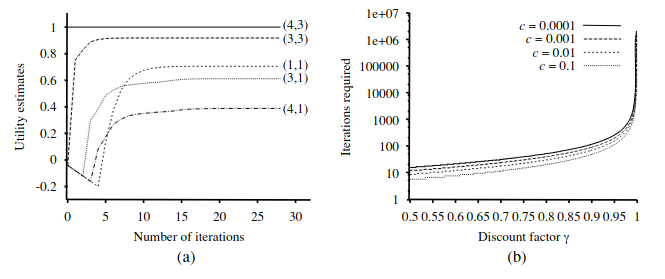
\includegraphics{images/image.png}
\caption{(a) Graph showing the evolution of the utilities of selected
states using value iteration. (b) The number of value iterations \(k\)
required to guarantee an error of at most
\(\epsilon = c \cdot R_{max}\), for different values of c, as a function
of the discount factor \gamma.}\label{fig:bellman_update}
}
\end{figure}

\hypertarget{partially-observable-mdps}{%
\section{Partially Observable MDPs}\label{partially-observable-mdps}}

\begin{itemize}
\item
  Instead of assuming al the information is available to us (i.e.~we can
  directly observe which state we're in), we consider when this is not
  the case. Thus, we have \textbf{Partially Observable MDP}.
\item
  Here, we add a \textbf{sensor model}, \(P(e|s)\) similar to the HMM,
  and a \textbf{belief state}, \(b(s)\). Then we can determine the next
  belief state, \(b'\) as follows,

  \[
  b'(s')=\alpha\,P(e\,|\,s')\sum_{s}\,P(s'\,|\,s,a)\,b(s)
  \]
\end{itemize}

\begin{quote}
The fundamental insight required to understand POMDPs is this: \emph{the
optimal action depends only on the agent's current belief state}. That
is, the optimal policy can be described by a mapping \(\pi^*(b)\) from
belief states to actions.
\end{quote}

\begin{itemize}
\item
  Since we do not know the current state, it would also no make sense to
  base the optimal policy on the true current state.
\item
  In conclusion, it means that an update on each time step would look as
  follows:

  \begin{enumerate}
  \def\labelenumi{\arabic{enumi}.}
  \tightlist
  \item
    Given the current belief state, \(b\), execute the action
    \(a=\pi^*(b)\).
  \item
    Receive the perceived evidence \(e\).
  \item
    Set the current belief state to \(\mathrm{Forward}(b, a, e)\).
  \item
    Go back to \emph{1}.
  \end{enumerate}
\item
  Now, the thing is that we don't know what evidence we will actually
  receive. Therefore, we should estimate what the possible evidence
  might be. Or, at least, have a method of determining how reliable our
  update method might be.
\item
  Let's first return to the probability of finding evidence, \(e\), with
  what we do know,

  \[
  \begin{align}
  P(e|a,b) &=\sum_{s'}P(e|a,s',b)P(s'|a,b) \\
           &=\sum_{s'}P(e|s')P(s'|a,b) \\
           &=\sum_{s'}P(e|s')\sum_{s}P(s'|s,a)b(s)
  \end{align}
  \]
\item
  Then, we can determine the probability of finding that particular next
  belief, \(b'\), from the \(\rm{Forward}\) function.

  \begin{equation}\protect\hypertarget{eq:belief_transition}{}{
  \begin{align}
  P(b'\mid b,a) &= P(b'\mid a,b) = \sum_{e}P(b'\mid e,a,b)P(e\mid a,b) \\
                &= \sum_{e}P(b'\mid e,a,b)\sum_{s'}P(e\mid s')\sum_{s}P(s'\mid s,a)b(s)
  \end{align}
  }\label{eq:belief_transition}\end{equation}
\item
  Furthermore, we can define a reward function for beliefs:
  \begin{equation}\protect\hypertarget{eq:belief_reward}{}{
  \rho(b) = \sum_s b(s) R(s)
  }\label{eq:belief_reward}\end{equation}
\item
  In conclusion, if we consider eq.~\ref{eq:belief_transition} the
  \textbf{belief transition} and eq.~\ref{eq:belief_reward} the
  \textbf{belief reward}, we have essentially reduced the POMDP to a
  normal MDP.
\end{itemize}

\hypertarget{value-iteration-for-pomdps}{%
\subsection{\texorpdfstring{\hl{Value Iteration for
POMDPs}}{Value Iteration for POMDPs}}\label{value-iteration-for-pomdps}}

\begin{itemize}
\item
  Value iteration can be described by the following function:

  \begin{equation}\protect\hypertarget{eq:value_iteration}{}{
  \alpha_{p}(s)=R(s)+\gamma\left(\sum_{s^{\prime}}P(s^{\prime}|\,s,a)\sum_{e}P(e|\,s^{\prime})\alpha_{p,e}(s^{\prime})\right)
  }\label{eq:value_iteration}\end{equation}
\end{itemize}

\hypertarget{monte-carlo-tree-search}{%
\section{Monte Carlo Tree Search}\label{monte-carlo-tree-search}}

\begin{itemize}
\item
  An important observation is that up until one we have tried to
  determine the optimal policy performing any action, a so-called
  \textbf{offline planning} strategy.
\item
  \textbf{Monte Carlo Tree Search (MCTS)} is an example of an
  \textbf{online planning} strategy and attempts to determine the best
  action to take by considering the transition function inferred by the
  action, \(R(a) = s\), as a tree and stochastically exploring it.
\item
  Long story short, MCTS works according to the following algorithm
  starting from the root of the tree, i.e.~the current state:

  \begin{enumerate}
  \def\labelenumi{\arabic{enumi}.}
  \item
    \textbf{Selection:} Select a child node using a selection strategy
    until a node with unexplored children is reached or a terminal state
    is encountered.
  \item
    \textbf{Expansion:} If the selected node has unexplored children
    (i.e., possible moves from the current state), expand the tree by
    adding one or more child nodes corresponding to these unexplored
    moves.
  \item
    \textbf{Simulation (Rollout):} Simulate a random or heuristic
    playout using a \textbf{rollout policy} from the newly added node
    (or from the selected node if it was already a terminal state) until
    a terminal state is reached. This is essentially a random sampling
    phase and represents a possible outcome of the game from the current
    position.
  \item
    \textbf{Backpropagation:} Update the statistics of the nodes along
    the path from the newly expanded or simulated node to the root. This
    typically involves updating the visit count and the total
    accumulated reward (or score) of the nodes.
  \item
    \textbf{Repeat:} Repeat steps 1 to 4 for a fixed number of
    iterations or until a time limit is reached.
  \item
    \textbf{Action Selection:} After the specified number of iterations,
    or when a computational budget is exhausted, choose the best move
    from the root node based on the node visit counts or other relevant
    statistics. This is usually the child node with the highest visit
    count, indicating it has been explored the most and has shown
    promising results.
  \end{enumerate}
\item
  The rollout policy has an incredible effect on the performance of the
  MCTS algorithm. One could consider a MCTS algorithm to be essentially
  a \emph{policy improvement operator}. That is, you give it a policy,
  and MCTS makes it better by applying additional search.
\item
  Pros and cons:

  \begin{itemize}
  \tightlist
  \item
    (\(+\)) Rapidly zooms in on promising regions
  \item
    (\(+\)) Can be used to improve policies
  \item
    (\(+\)) Basis of many successful applications
  \item
    (\(-\)) Needle in the hay-stack problems
  \item
    (\(-\)) Problems with high branching factor
  \end{itemize}
\end{itemize}

\hypertarget{reinforcement-learning}{%
\chapter{Reinforcement Learning}\label{reinforcement-learning}}

The general idea of reinforcement learning comes down to the fact that
we don't know exactly what the agent should do, but we do know when it
has done something right. While we don't know \emph{how} to win a chess
game, we do know the goal is to win. Therefore, \textbf{Reinforcement
Learning (RL)} concerns itself with learning based on \textbf{rewards}.

\begin{itemize}
\item
  We will specifically consider 3 designs:

  \begin{enumerate}
  \def\labelenumi{\arabic{enumi}.}
  \item
    A \textbf{utility-base} agent that learns a utility function based
    on the states and from there behaves to maximize its utility.
    \hl{This seems similar to the utility of a state from the MDP
    chapter.}
  \item
    A \textbf{Q-Learning} agent that learns an \textbf{action-utility},
    or \textbf{Q-function}, giving the expected utility of taking an
    action in a certain state.
  \item
    A \textbf{reflex agent} that learns a policy that maps directly from
    states to actions. \hl{In MDPs from the previous chapter this was
    the first introduced technique I think}
  \end{enumerate}
\item
  Generally, there are two variants: \textbf{passive} learning, where a
  policy is fixed and an agent learns the utilities of the states; and
  \textbf{active} where is learns the utilities as well as the policy.
\item
  In all cases, the primary problem is for the agent to \textbf{explore}
  as much of the domain. The agent needs to have had an adequate number
  of experiences to take sufficiently informed actions. That is, an
  agent should refrain from \textbf{beunen}.
\end{itemize}

\begin{figure}
\hypertarget{fig:very_import}{%
\centering
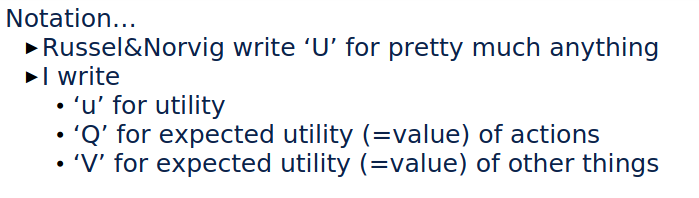
\includegraphics{images/image-1.png}
\caption{I guess this might be important for the
exam}\label{fig:very_import}
}
\end{figure}

\begin{itemize}
\tightlist
\item
  There is also a distinction to be made between \textbf{model-free} and
  \textbf{model-based} reinforcement learning.

  \begin{itemize}
  \tightlist
  \item
    \textbf{Model-free} learning captures learning methods which do not
    take into account the underlying transition and reward functions,
    \(P\) and \(R\) resp, of the underlying MDP.
  \item
    \textbf{Model-based} RL attempts to populate these functions with
    learned values or distributions.
  \end{itemize}
\end{itemize}

\hypertarget{model-free-reinforcement-learning}{%
\section{Model-Free Reinforcement
Learning}\label{model-free-reinforcement-learning}}

\hypertarget{passive-learning}{%
\subsection{Passive Learning}\label{passive-learning}}

\begin{itemize}
\item
  The most simple example is that of a passive, model-free agent in a
  state-based representation where are the environment is fully
  observable.
\item
  The policy is fixed, so we will determine the utility of the policy.
\item
  The big difference being a lack of a \textbf{transition model},
  \(P(s' \bar s,a)\), and \textbf{reward function}, \(R(s)\).
\item
  The first method is \textbf{direct utility estimation} (aka
  \textbf{Monte Carlo prediction}) which basically boils down to
  executing the policy many times starting from a new state each time.
  From this, we get an expected reward that represents the utiltiy of
  the state.
\item
  It is \textbf{unbiased}, meaning it will converge to the right
  solution, but has high \textbf{variance}, meaning it will take a lot
  of samples to get there.
\item
  A problem with this is that is doesn't take into account that the
  utility of the current state is dependent on that of the previous
  according to the bellman equation.
\item
  An alternative is to use \textbf{temporal-difference} learning which
  expresses the utility of the `current' state into that in a difference
  between it and successive states. Formally, it uses the following
  relation to update the utility of the current state, given the current
  policy.

  \begin{equation}\protect\hypertarget{eq:td_update}{}{
  U^\pi(s) \leftarrow U^\pi(s) + \alpha(R(s) + \gamma U^\pi(s') - U^\pi(s))
  }\label{eq:td_update}\end{equation}

  Here, \(\alpha\) is the \textbf{learning rate}.
\item
  It could be considered a form of \textbf{stochastic gradient descent
  (SGD)}, but not quite. \hl{Not exactly sure why not quite. It's not
  very clear from the slides.}
\item
  It's important to note that this method is \textbf{biased} due to
  \textbf{bootstrapping}, but has \textbf{lower variance} than the
  previous method. The \textbf{bootstrapping} comes from the assumption
  in eq.~\ref{eq:td_update} that this holds even for non-final
  \(U^\pi(s)\).
\end{itemize}

\hypertarget{active-learning}{%
\subsection{Active Learning}\label{active-learning}}

\begin{itemize}
\item
  We know how to learn \(U^\pi\), but we really want to know how to
  learn \(U^*\). Therefore, we have to learn a policy.
\item
  A very simple approach would be to adapt eq.~\ref{eq:td_update} to use
  \(U(s, a)\) instead:

  \begin{equation}\protect\hypertarget{eq:q_update}{}{
  U^\pi(s, a) \leftarrow U^\pi(s, a) + \alpha(R(s, a) + \gamma \max_{a'} U^\pi(s', a') -
  U^\pi(s, a))
  }\label{eq:q_update}\end{equation}

  The expected utility of a state-action pair is also often denoted as
  \(Q\). Therefore, this approach is also called \textbf{Q-Learning}.
  Note that we are taking \(a'\) with that returns the maximum utility.
\item
  \textbf{State-action-reward-state-action (SARSA)} is an alternative to
  the prior where we don't take the max action. We then essentially
  determine the expected utility of a policy. We can then try to
  optimize such that \(\pi \rightarrow \pi^*\).
\end{itemize}

\hypertarget{scaling-up}{%
\subsection{Scaling Up}\label{scaling-up}}

\begin{itemize}
\item
  Up until now, we have solely worked in a state-action based system
  which is essentially represented by a lookup table. Performing the
  previous algorithms on large state-spaces, however, quickly becomes
  impractical.
\item
  An alternative to such a tabular approach would be \textbf{function
  approximation}. That is, use any sort of function to approximate the
  model. One such example would be to use a neural network.
\item
  It's not `true' gradient descent so only a few of the nice properties
  associated with it remain (at least for linear functions):

  \begin{itemize}
  \tightlist
  \item
    TD learning: \textbf{converges} to bounded approximation.
  \item
    SARSA: might \textbf{chatter} (cycle around the optimal solution)
    but not diverge.
  \item
    Q-learning: can \textbf{diverge}.
  \end{itemize}
\item
  The last property can be attributed to the \textbf{deadly triad of
  RL}:

  \begin{enumerate}
  \def\labelenumi{\arabic{enumi}.}
  \tightlist
  \item
    bootstrapping,
  \item
    off-policy learning, and
  \item
    function approximation
  \end{enumerate}
\end{itemize}

\hypertarget{policy-search}{%
\subsection{Policy Search}\label{policy-search}}

\begin{itemize}
\item
  \textbf{Policy search} is very simple: just keep changing the policy
  until it improves, then stop. An example would be the following:

  \[
  \pi(s)=\operatorname*{max}_{a}Q_{\theta}(s,a)
  \]

  The idea is then that policy search would adjust the parameters,
  \(\theta\), such that the policy improves.
\item
  The policy could be improved by determining the \textbf{policy
  gradient} from the \textbf{policy value} and applying a hill-climbing
  algorithm.
\item
  This could be combined with a value function that evaluates the
  current policy, in something called an \textbf{actor-critic method}.
  This reduces high variance otherwise associated with policy gradient
  methods.
\end{itemize}

\hypertarget{model-based-reinforcement-learning}{%
\section{Model-Based Reinforcement
Learning}\label{model-based-reinforcement-learning}}

\backmatter
\end{document}
